\chapter{Scattering simulation}
\label{scattering}
Finally after all our hard work of investigating the dispersion curves of
different lattices as well as finding out how to perturb them such that we form
a bandgap, we will actually simulate how a wave of a certain frequency
propagates and scatters through a finite portion of one of our lattices.

Similarly to how we joined cells together to from a strip, we will do the same
and join strips to form a finite lattice. We may then reframe our eigen-problem
systems in reciprocal space into linear systems in physical space. From there,
we can solve the linear systems to see how the energy or wave moves throughout
the entire space. All we need to do is pick a frequency for the wave we want to
simulate as well as where we want the source of excitation to be.

From the dispersion relations, we know which frequency waves are able to
propagate across the lattice and which frequencies are not transmitted through
the lattice. As we have discussed before in Chapter \ref{formstrip}, we know
that there are certain frequencies which are only able to propagate along the
interface of the strips and not anywhere else in the lattice. These are the
frequencies which we will be simulating.

\section{Our linear system in physical space}
Before we can run our scattering simulations, which essentially is solving for
the displacements of masses in our finite lattice, we need to form the system
to solve. This actually turns out to be really similar to the eigen-problems we
had earlier (albeit with a much larger matrix involved!). It is also useful to
note that the following derivation works just as well for systems of any shape
as long as we have formed the eigen-problem as before, as we will reuse the
variables in the eigen-problem here.
 
The key idea in this is that we can pick and choose the frequency, $\Omega$,
and so by just
%TODO: Finish derivation of linear system

With this linear system set up, let us take a look at the physical spaces in
which we will run these simulations.

\section{2d hexagonal finite lattice}
\begin{figure}[!h]
\centering
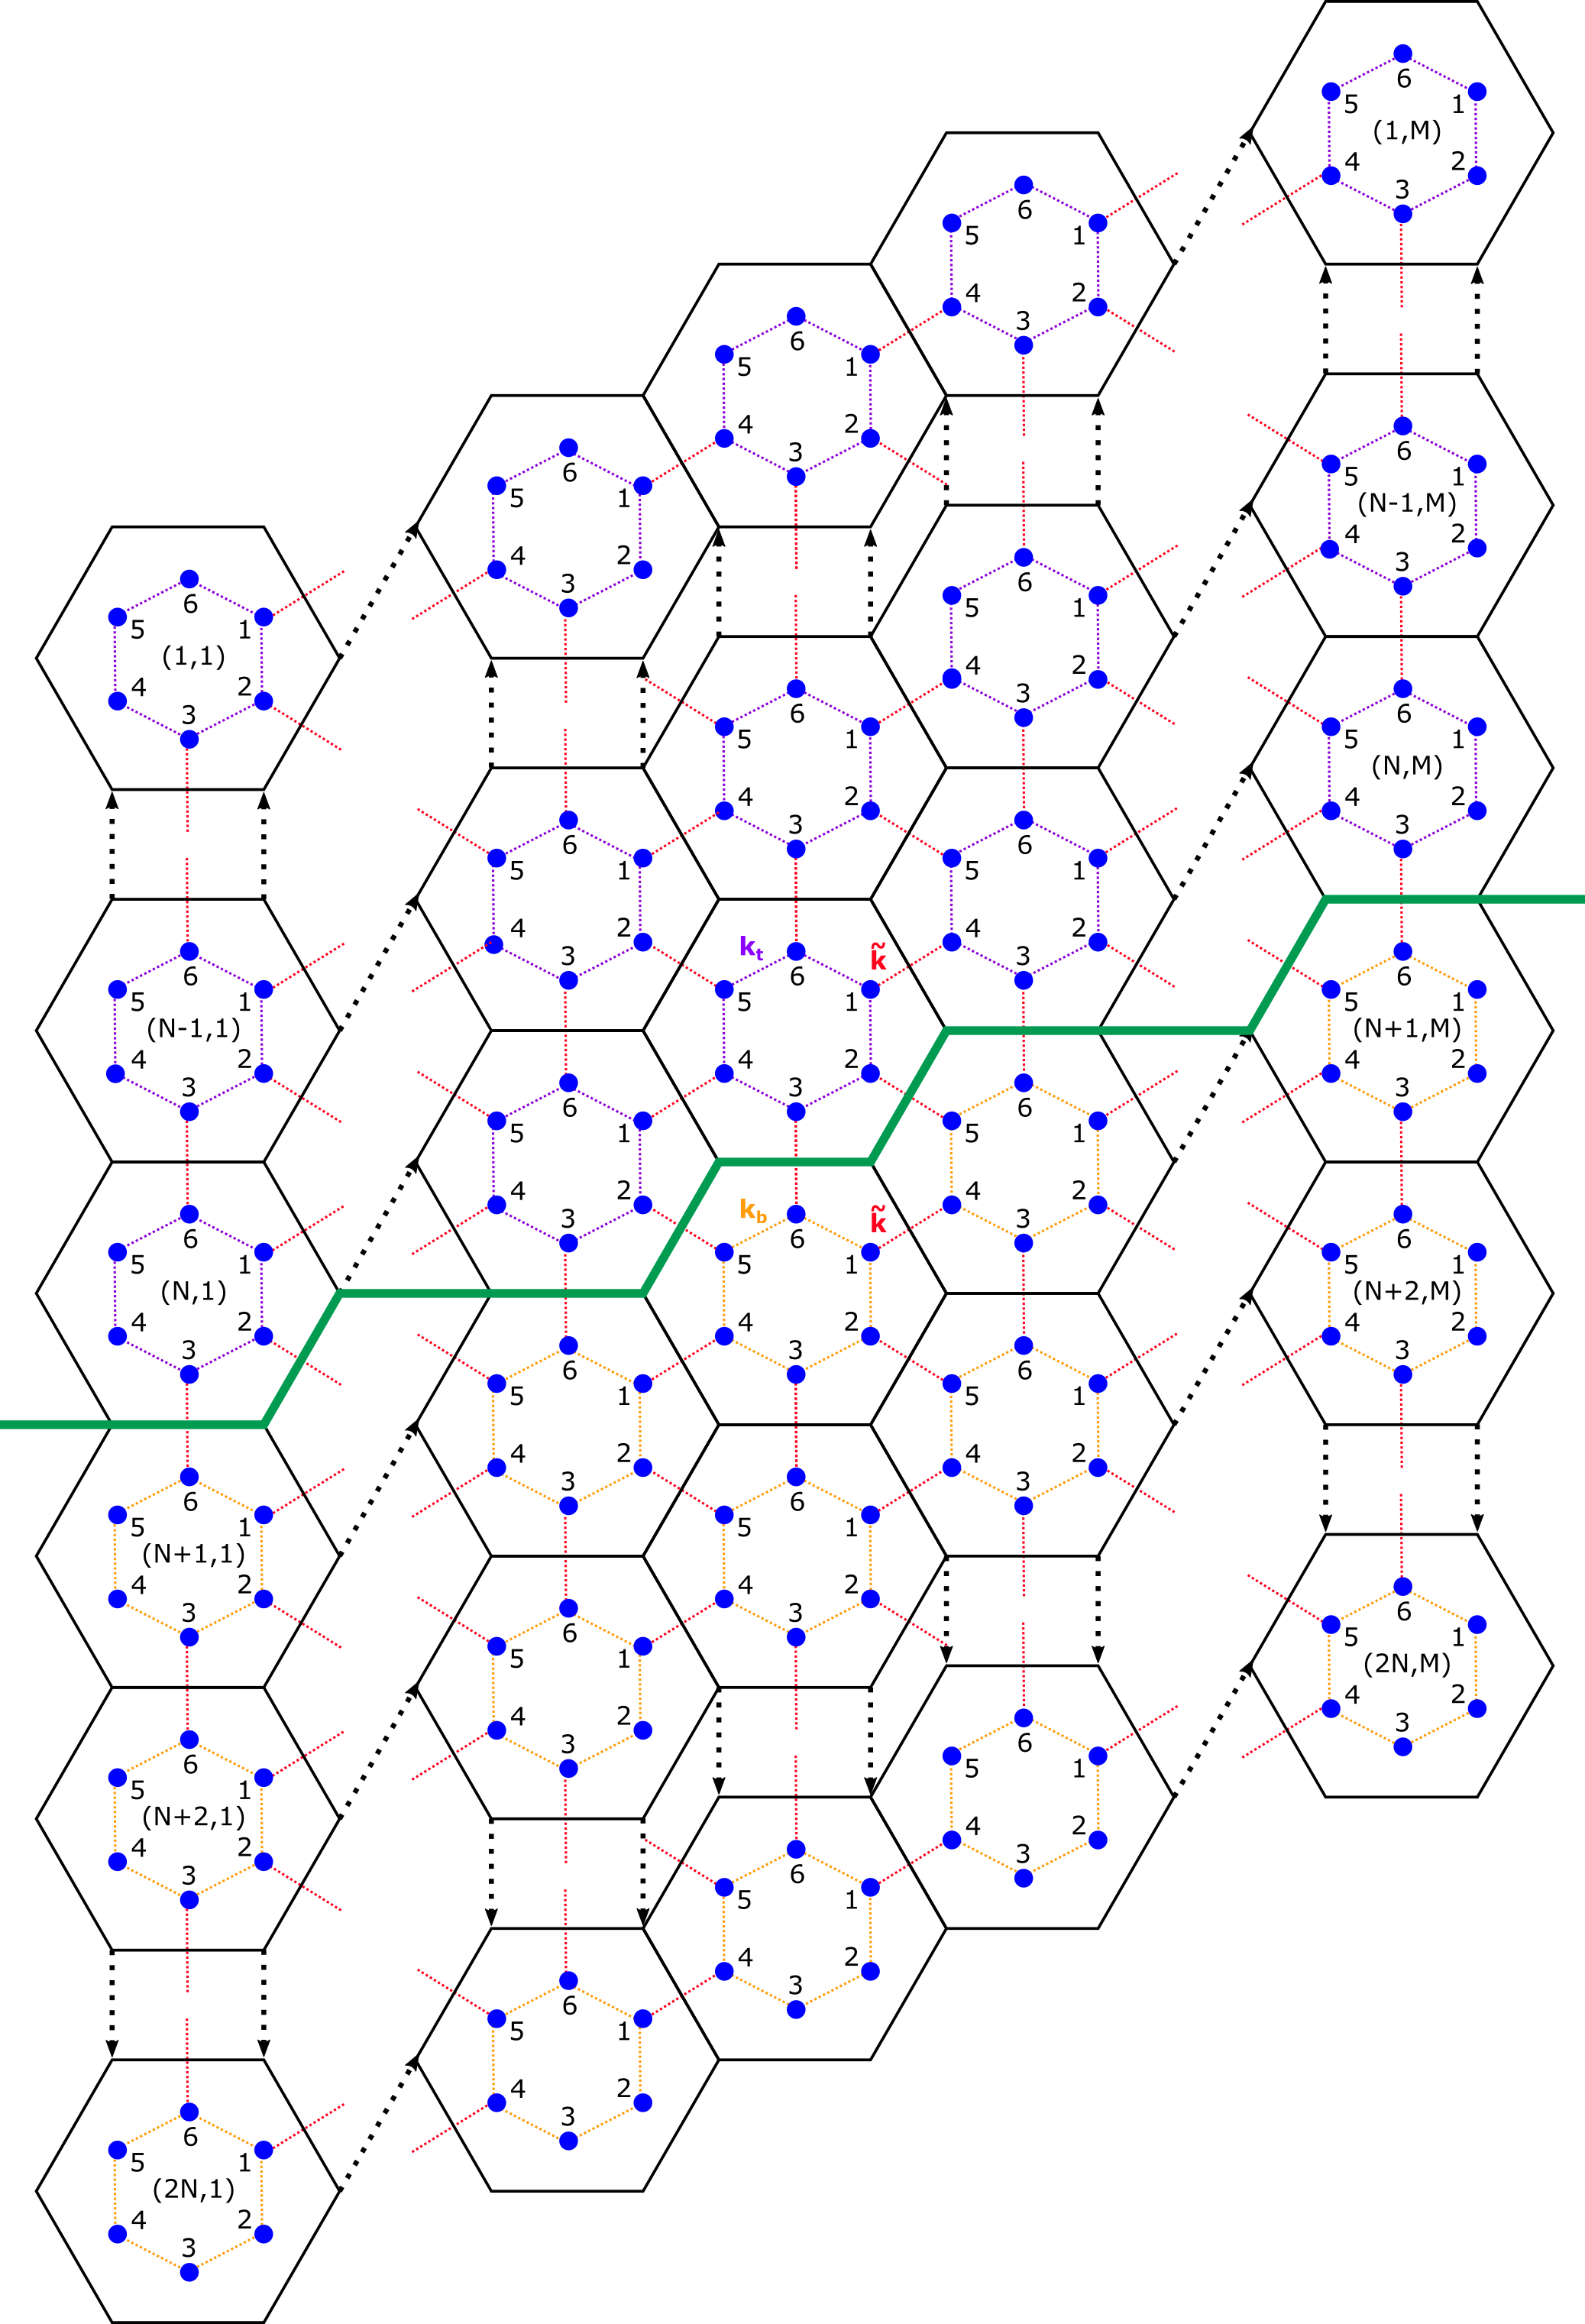
\includegraphics[width=0.8\textwidth]{imgs/hexfinitemodel.png}
\caption{\label{fig:hexfinscheme} Schematic view of the finite hexagonal
  lattice formed from the joining of strips side-by-side, where the strips
  themselves are formed from two different halves as in Chapter
  \ref{perturbed}.  Note the conditions imposed at the boundaries (masses at
  boundaries have no connections outside the lattice).}
\end{figure}

Specifically, we will be running our following simulations on the arrangement
of cells in Figure~\ref{fig:hexstdfinlattice}.

\begin{figure}
  \centering
  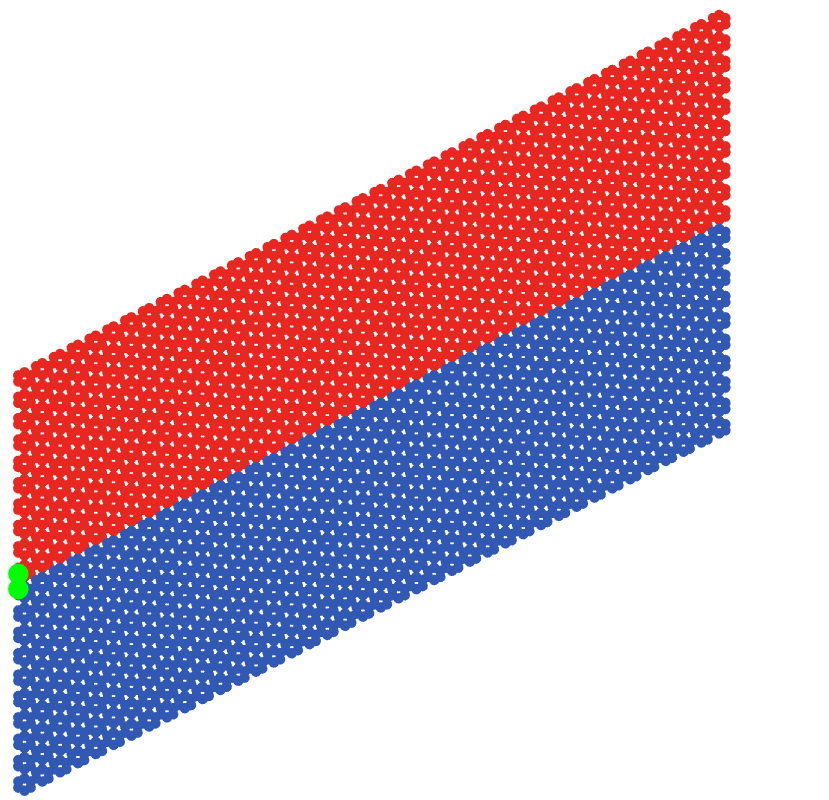
\includegraphics[width=0.5\linewidth]{imgs/hexstdfinlattice.png}
  \caption{Arrangement of hexagonal cells ($2N=20$, $M=40$), with red and blue
    being different materials, and source of excitation at the green masses.}
  \label{fig:hexstdfinlattice}
\end{figure}

\subsection{Alternating masses}

In this section we will run scattering simulations on the physical lattice as
described in Chapter \ref{perturbaltmass} with the alternating masses.

Now, we can run our simulations for another frequency we want, but we know from
our dispersion relations that most frequencies (those outside the special
dispersion curves corresponding to the edge states) will just propagate
throughout the lattice and so we would not get any discernible patterns of
movement. An example can be found in Figure~\ref{fig:randscat}.

\begin{figure}
\centering
\begin{subfigure}[b]{.5\textwidth}
  \centering
  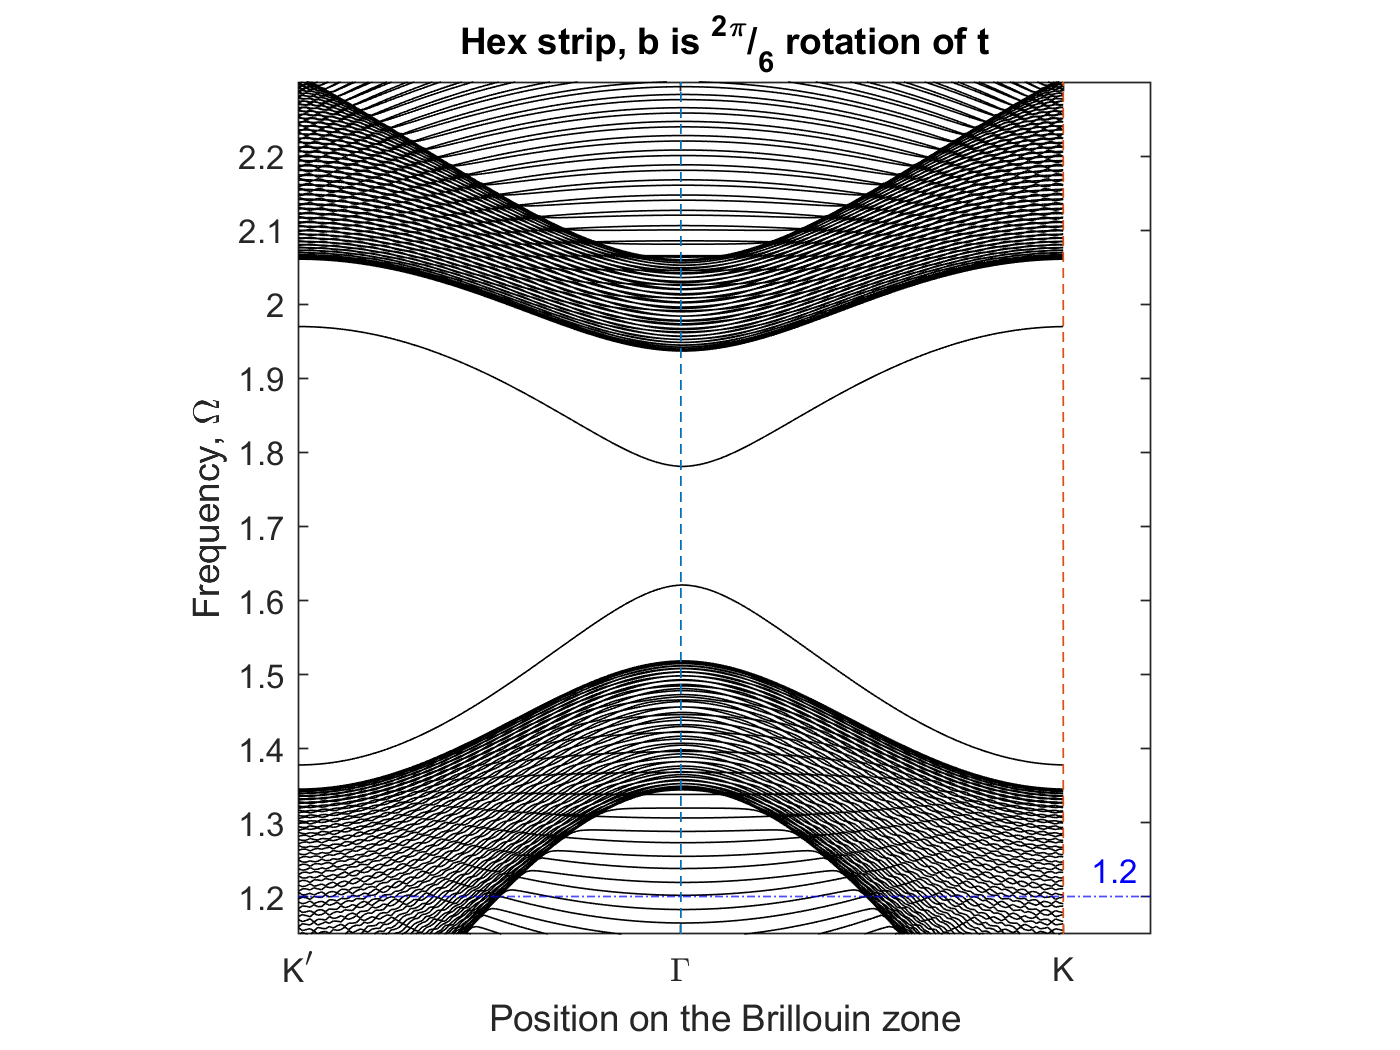
\includegraphics[width=1.1\linewidth]{imgs/hexstripperturbMrotatedrand.png}
  \caption{Zoomed in look of Figure~\ref{fig:hexstripMrotated} near the bandgap.}
\label{fig:sub1}
\end{subfigure}%
\begin{subfigure}[b]{.5\textwidth}
  \centering
  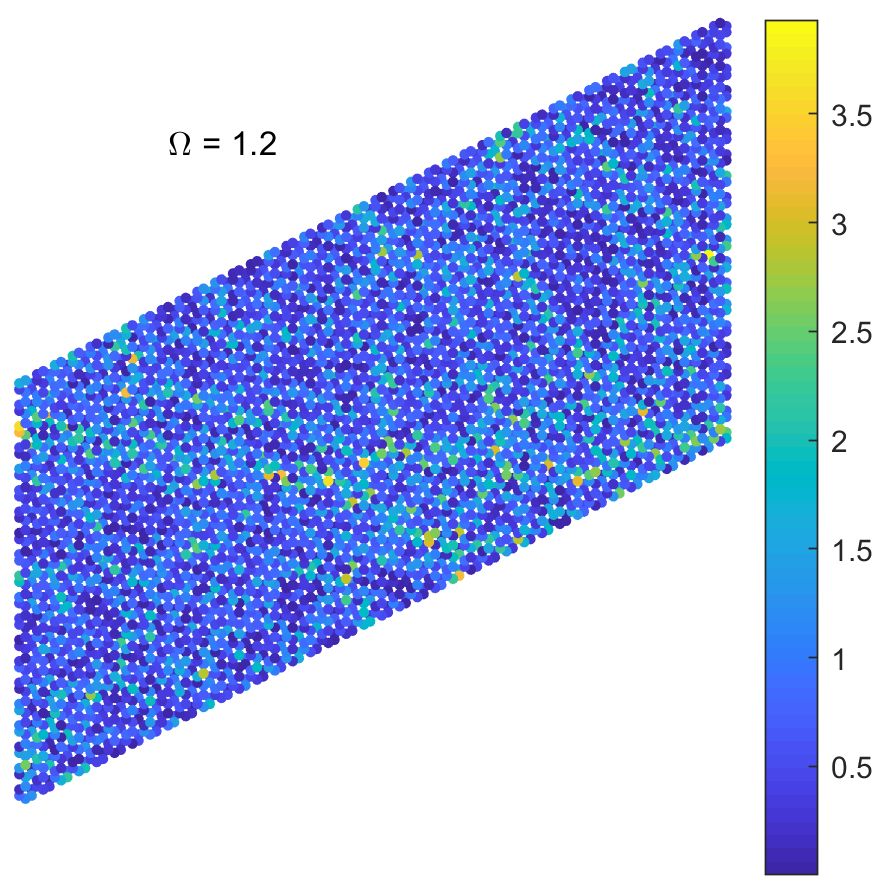
\includegraphics[width=1\linewidth]{imgs/hexstdrandscat.png}
  \caption{The plot of $|y_i|$ for each mass in each cell.}
  \label{fig:sub2}
\end{subfigure}
\caption{Simulation of scattering on the hexagonal finite lattice in
  Figure~\ref{fig:hexstdfinlattice} with the alternating masses as defined in
  Figure~\ref{fig:hexstripMrotated} with $\Omega = 1.2$.}
\label{fig:randscat}
\end{figure}

As we are interested in being able to direct waves to our liking, it is much
more exciting to fire a frequency which is only able to travel along the
boundary. So let use the same system as in Figure~\ref{fig:randscat} again, but
using $\Omega = 1.6$ instead as we can see in
Figure~\ref{fig:hexstripMrotatedzooms1} that the dispersion curve for that edge
mode lives in the bandgap.

\begin{figure}
\centering
\begin{subfigure}[b]{.5\textwidth}
  \centering
  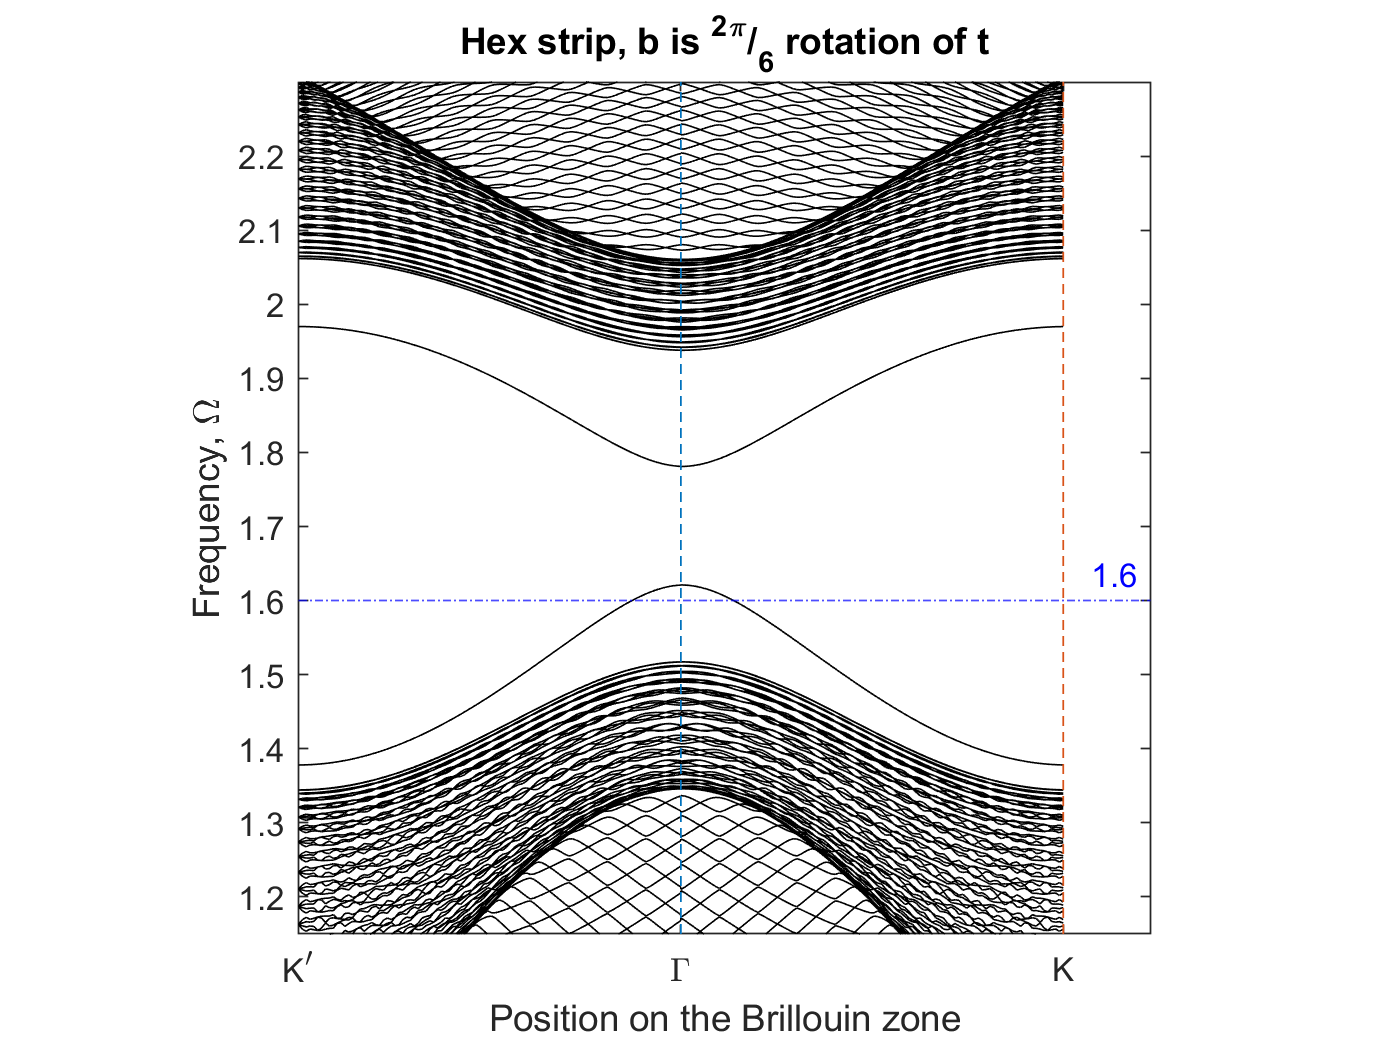
\includegraphics[width=1.1\linewidth]{imgs/hexstripperturbMrotatedzoom.png}
  \caption{Zoomed in look of Figure~\ref{fig:hexstripMrotated} near the bandgap.}
  \label{fig:hexstripMrotatedzooms1}
\end{subfigure}%
\begin{subfigure}[b]{.5\textwidth}
  \centering
  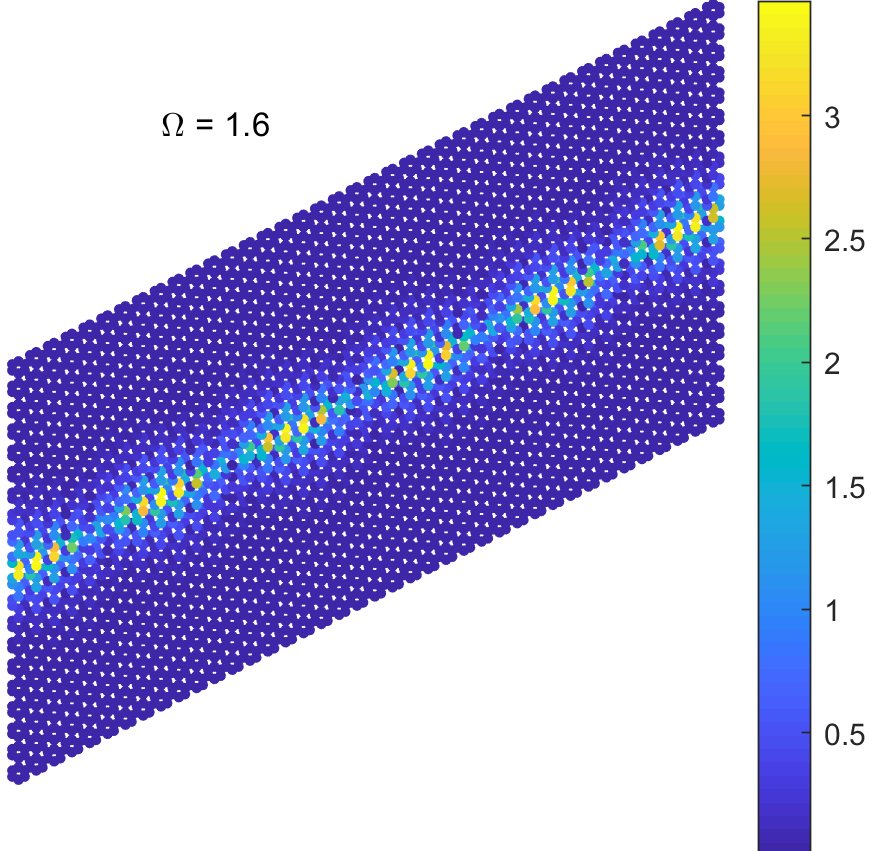
\includegraphics[width=1\linewidth]{imgs/hexstdrotstraight.png}
  \caption{The plot of $|y_i|$ for each mass in each cell.}
  \label{fig:sub2}
\end{subfigure}
\caption{Simulation of scattering on the hexagonal finite lattice in
  Figure~\ref{fig:hexstdfinlattice} with the alternating masses as defined in
  Figure~\ref{fig:hexstripMrotated} with $\Omega = 1.6$.}
\label{fig:hexstdrotstraight}
\end{figure}

Wonderful! Finally after all our hard work we can see in
Figure~\ref{fig:hexstdrotstraight} that the wave or energy forced into the
system is only propagating along the straight line. This effectively means that
we can control the direction of propagation of waves through our lattice and
not have it diffuse or \textit{leak} out into the other parts of the lattice.
Of course our next thought would be to see if it is possible to send the energy
around bends and more complex boundaries, which is what we discuss in Chapter
\ref{complexbends}.

\subsection{Varying mass and stiffnesses}
In this section we will take a look at running scattering simulations as above
but for the physical system discussed in Chapter \ref{perturbMk}.

\begin{figure}
\centering
\begin{subfigure}[b]{.5\textwidth}
  \centering
  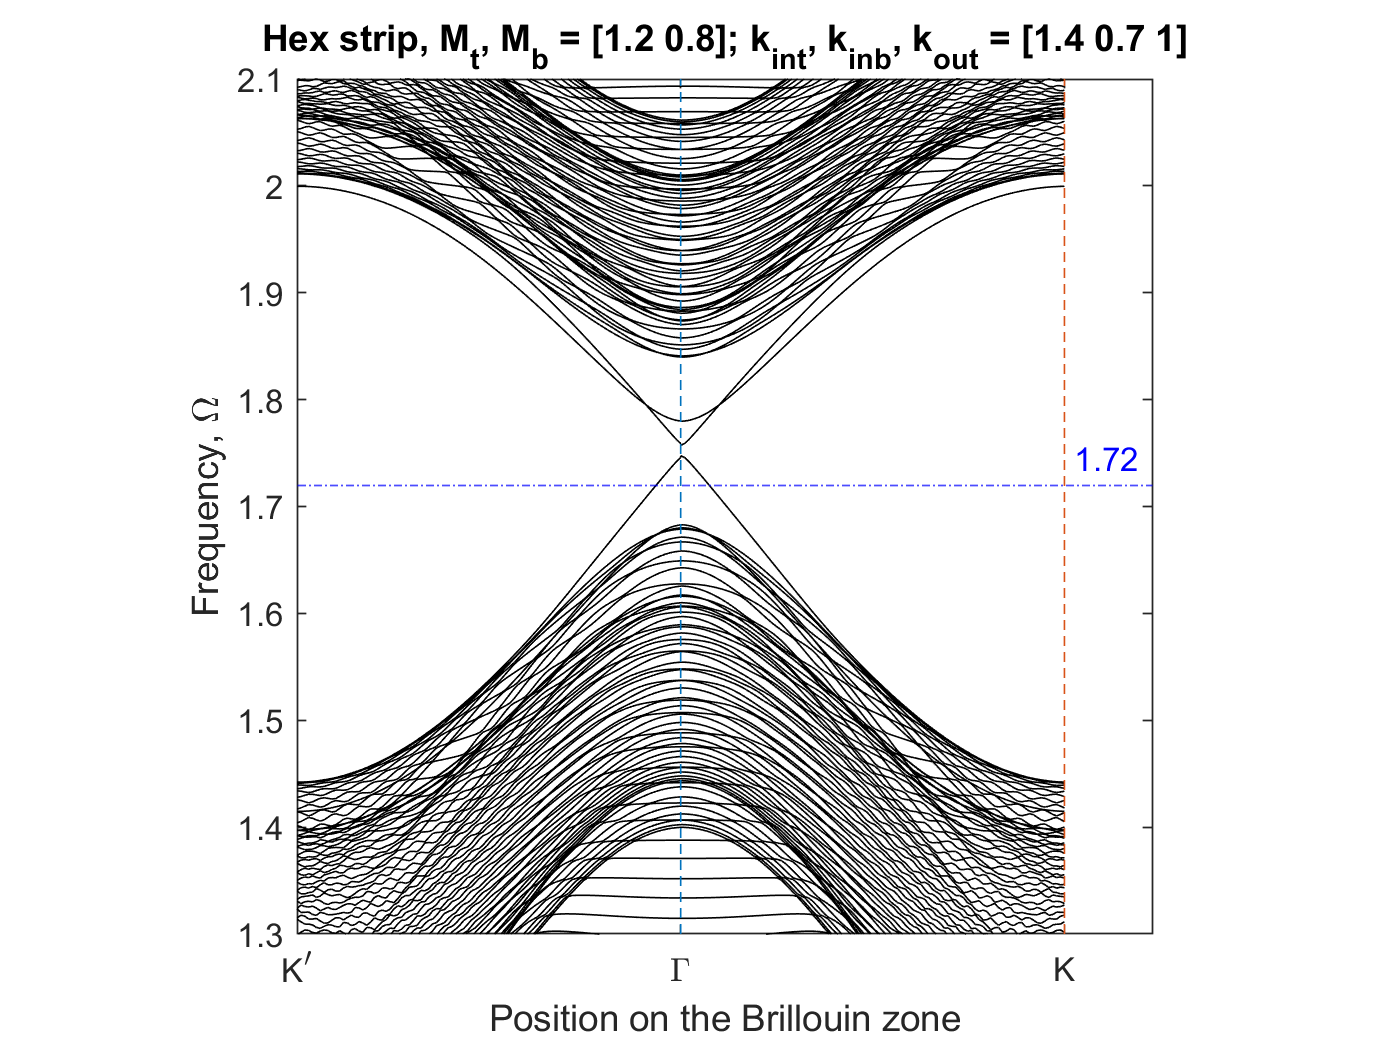
\includegraphics[width=1.1\linewidth]{imgs/hexstripperturb2zoom.png}
  \caption{Zoomed in look of Figure~\ref{fig:hexstrip2} near the bandgap.}
  \label{fig:sub1}
\end{subfigure}%
\begin{subfigure}[b]{.5\textwidth}
  \centering
  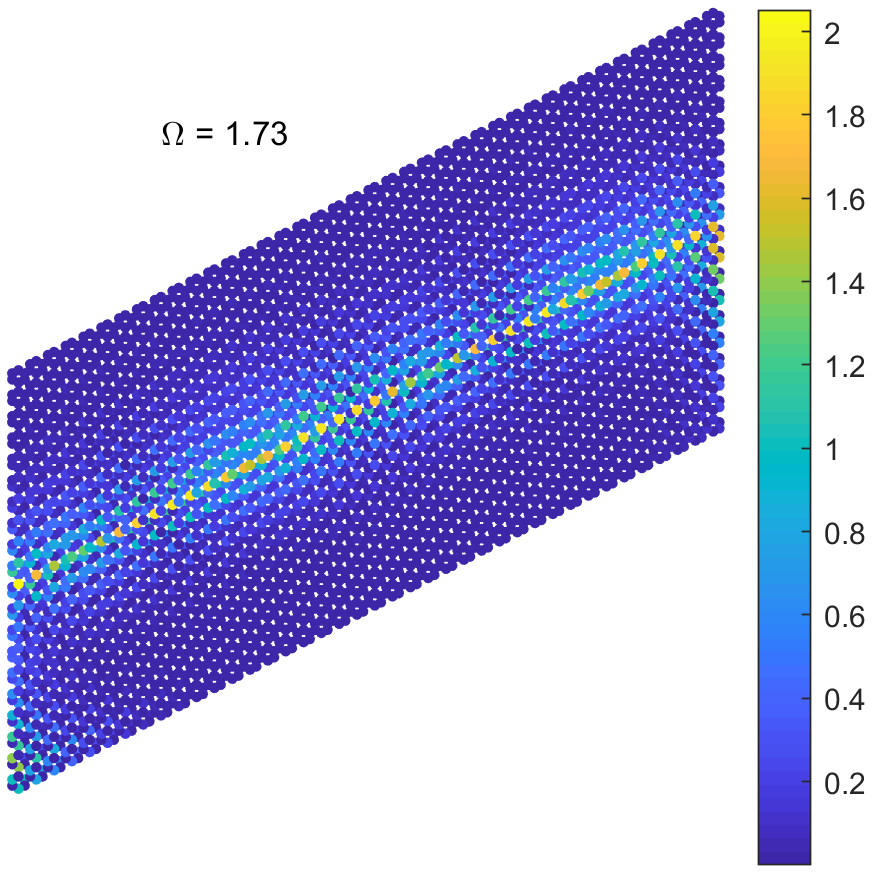
\includegraphics[width=1\linewidth]{imgs/hexstdMk.png}
  \caption{The plot of $|y_i|$ for each mass in each cell.}
  \label{fig:sub2}
\end{subfigure}
\caption{Simulation of scattering on the hexagonal finite lattice in
  Figure~\ref{fig:hexstdfinlattice} with the top having a greater $M$ and $k$
  than the bottom as defined in Figure~\ref{fig:hexstrip2} with $\Omega =
  1.72$.}
\label{fig:hexstdMk}
\end{figure}

\section{2d kagome finite lattice}
\begin{figure}[!h]
\centering
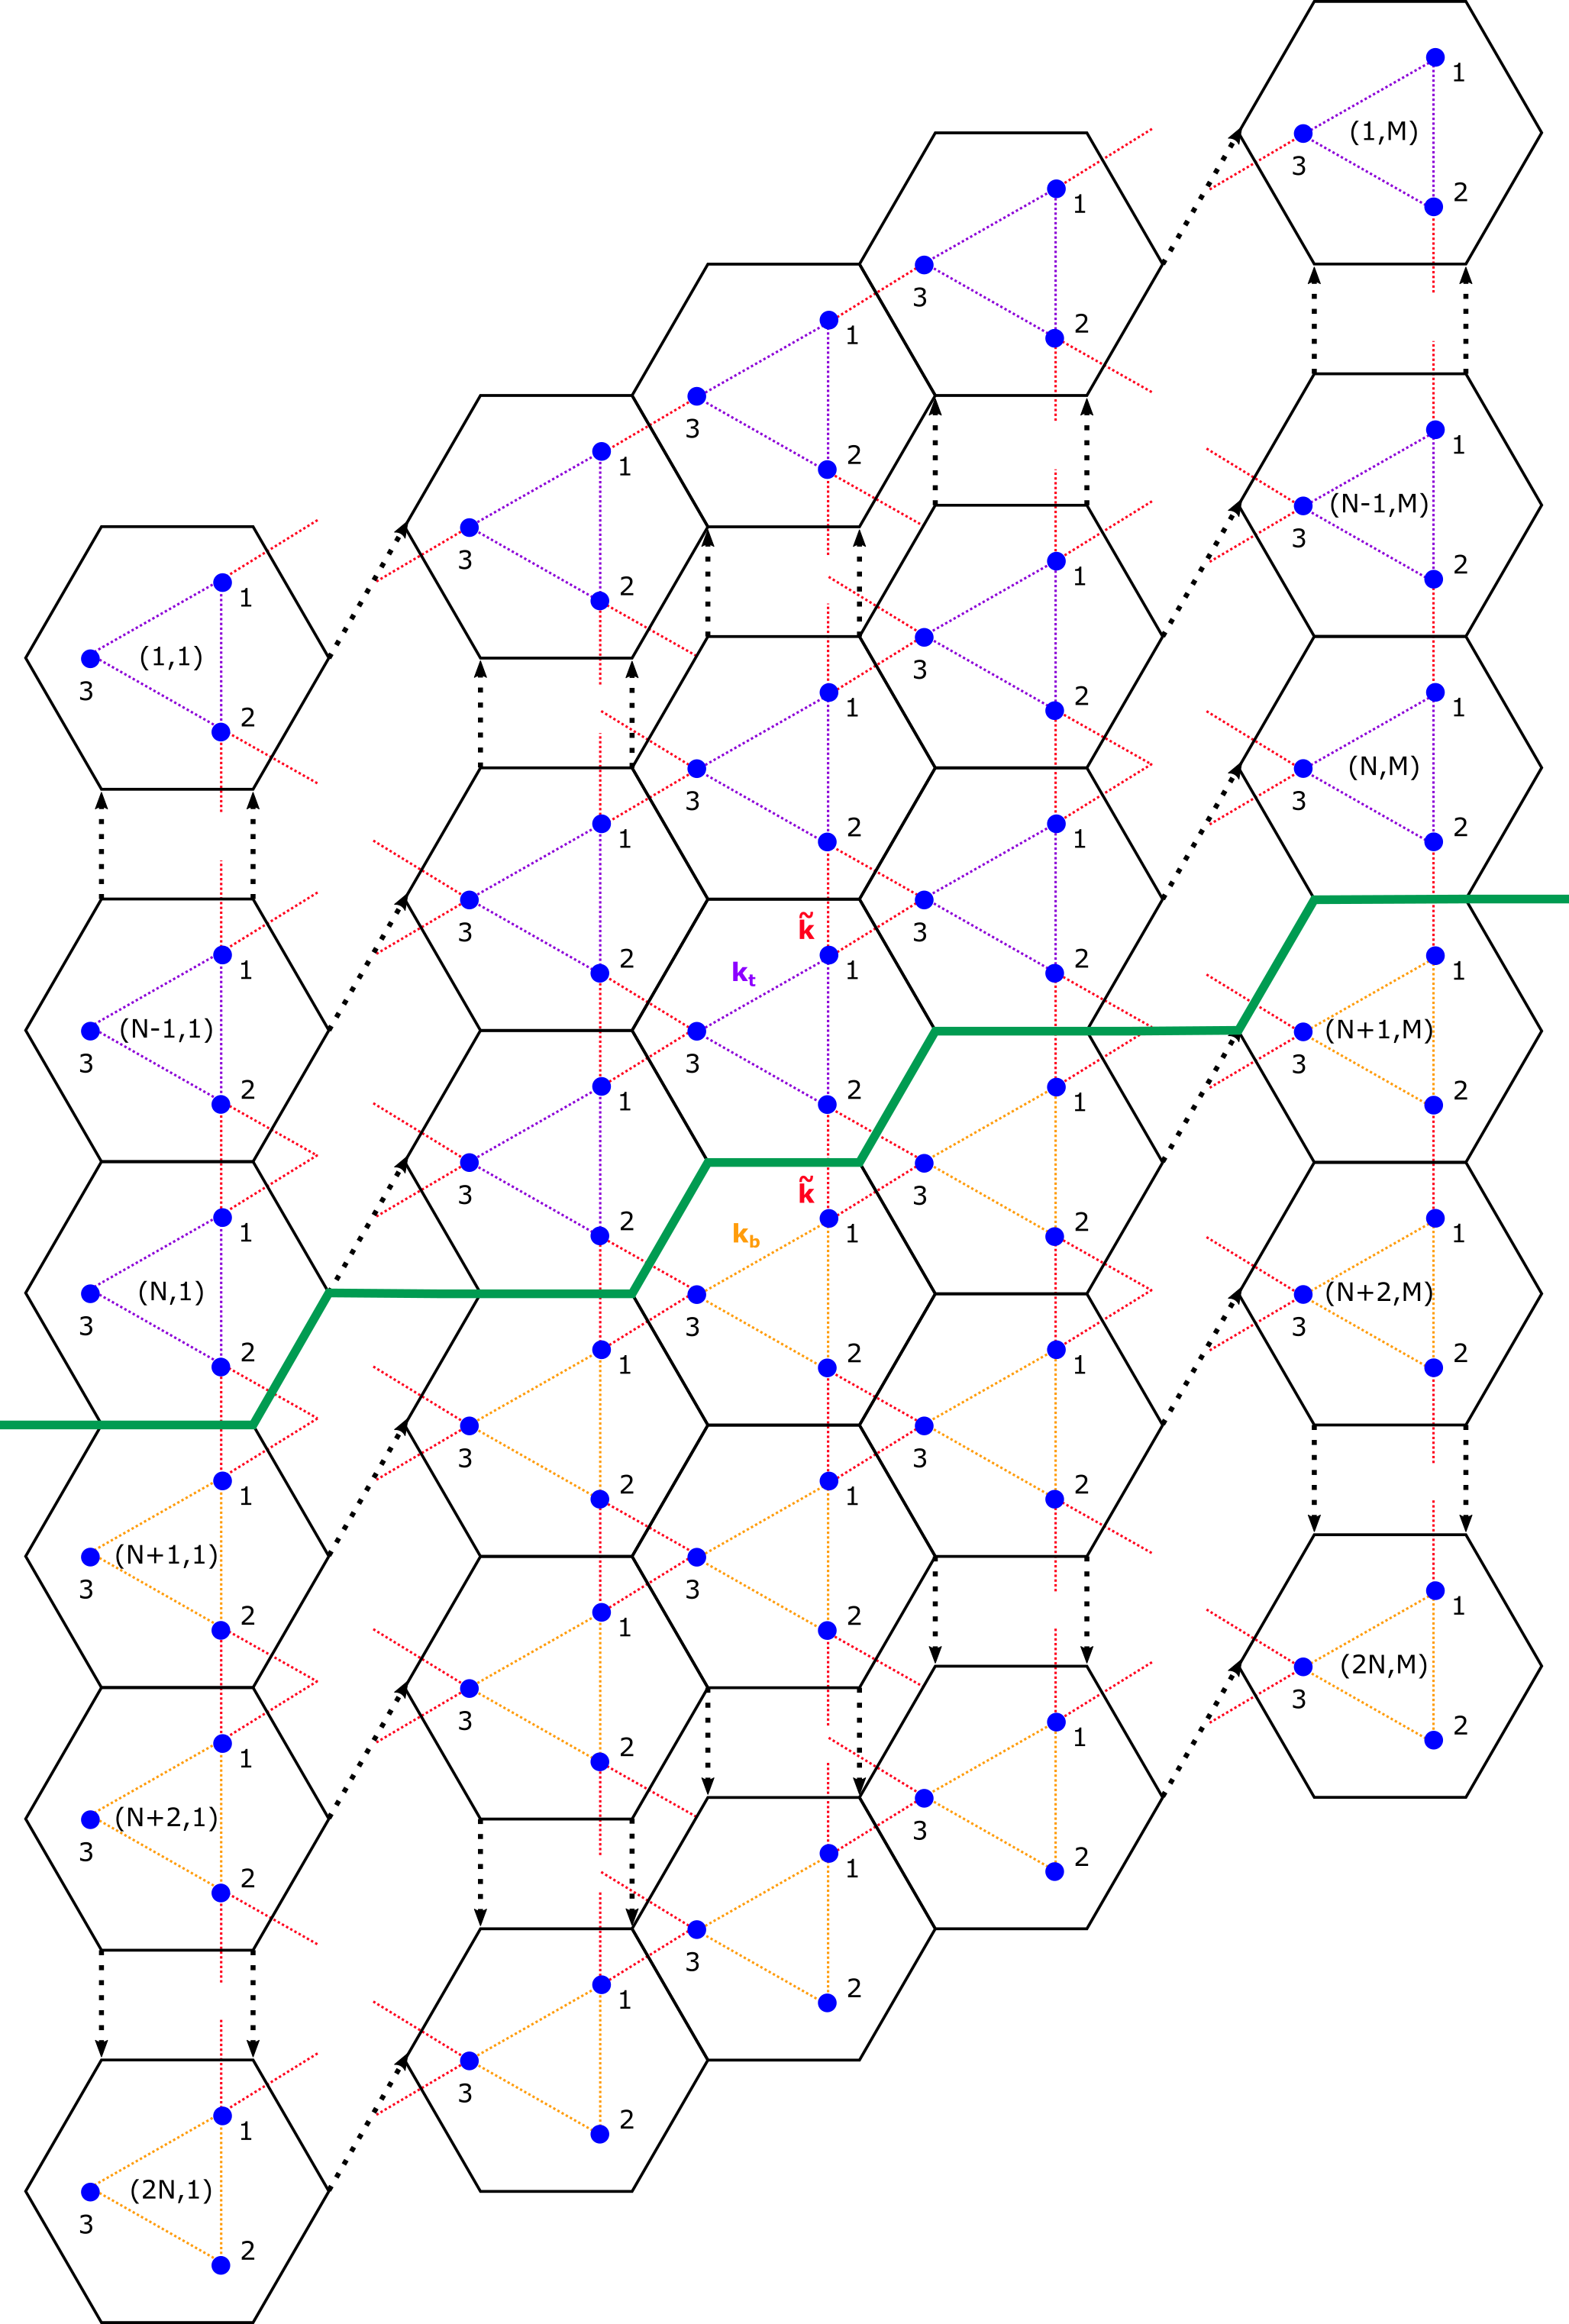
\includegraphics[width=0.8\textwidth]{imgs/kagomefinitemodel.png}
\caption{\label{fig:kagomefinscheme} Schematic view of the finite kagome
  lattice formed from the joining of strips side-by-side, where the strips
  themselves are formed from two different halves as in Chapter
  \ref{perturbed}. Note the conditions imposed at the boundaries (masses at
  boundaries have no connections outside the lattice).}
\end{figure}

\section{Complex bends}
\label{complexbends}
Now that we have built up the foundation of how we can force a wave to
propagate in a specific direction in a topologically repeating material or
metamaterial, we want to see just how robust this phenomenon is based on the
shape of the boundary, i.e. just how much can we bend the wave?

\textit{Note:}Since we have already shown that this can be done for both the
hexagonal and kagome lattice, in this section we will only be running our
simulations for the hexagonal lattice to avoid duplication, as we are just
exploring whether the shape of the boundary affects the scattering.
Furthermore, we will specifically be using the same top and bottom cels as
Figure~\ref{hexstdrotstraight}, which is with alternating masses as defined in
Figure~\ref{fig:hexstripMrotated}.

\subsection{Gentle and sharp straight bends}
So far we have seen just straight line boundaries, but can this work for bent
boundaries too? Due to the way we set up our lattice (with the strips getting
higher as we go from left to right), there are two kinds of bends we can make
straight away. The 'gentle' bend where we bend the boundary upwards, and the
'sharp' bend where we bend the boundary downwards.

\begin{figure}
\centering
\begin{subfigure}[b]{.5\textwidth}
  \centering
  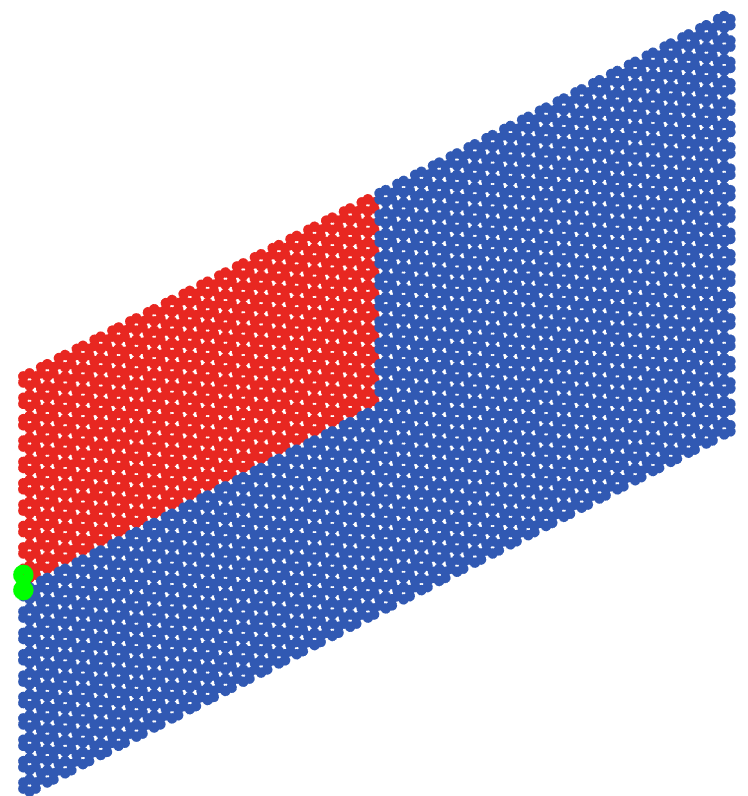
\includegraphics[width=0.8\linewidth]{imgs/gentlebendarr.png}
  \caption{Arrangement of cells to form a gentle bend.}
  \label{fig:sub1}
\end{subfigure}%
\begin{subfigure}[b]{.5\textwidth}
  \centering
  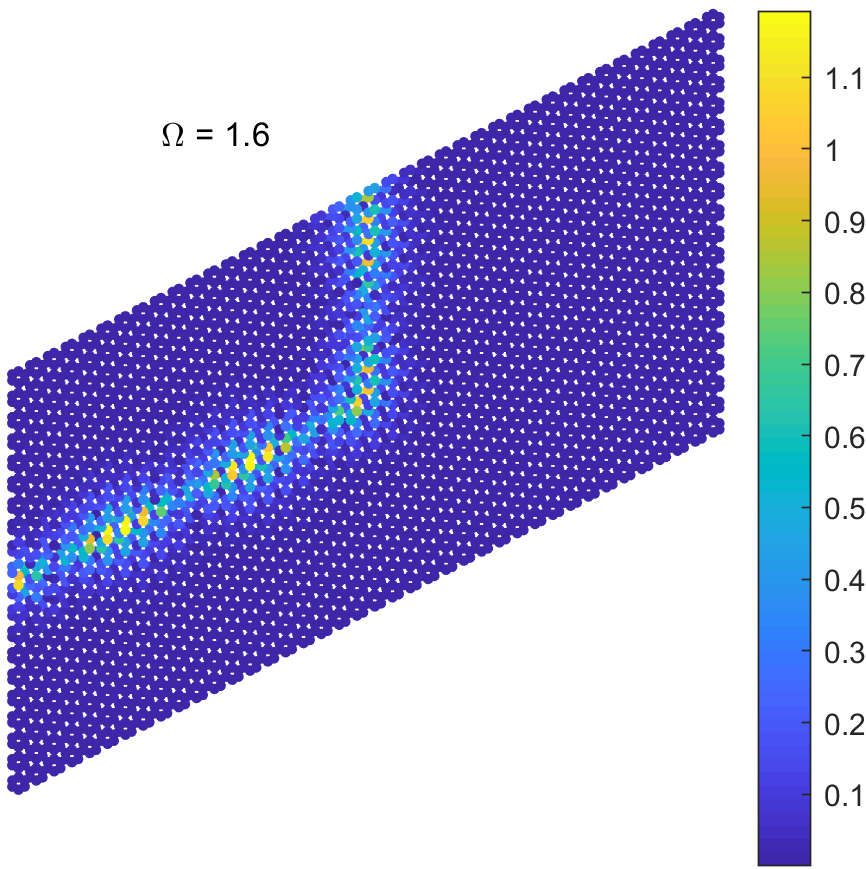
\includegraphics[width=1\linewidth]{imgs/gentlebendscat.png}
  \caption{The plot of $|y_i|$ for each mass in each cell.}
  \label{fig:sub2}
\end{subfigure}
\caption{Simulation of scattering on the hexagonal finite lattice with gentle
  bend.}
\label{fig:gentlebend}
\end{figure}

\begin{figure}
\centering
\begin{subfigure}[b]{.5\textwidth}
  \centering
  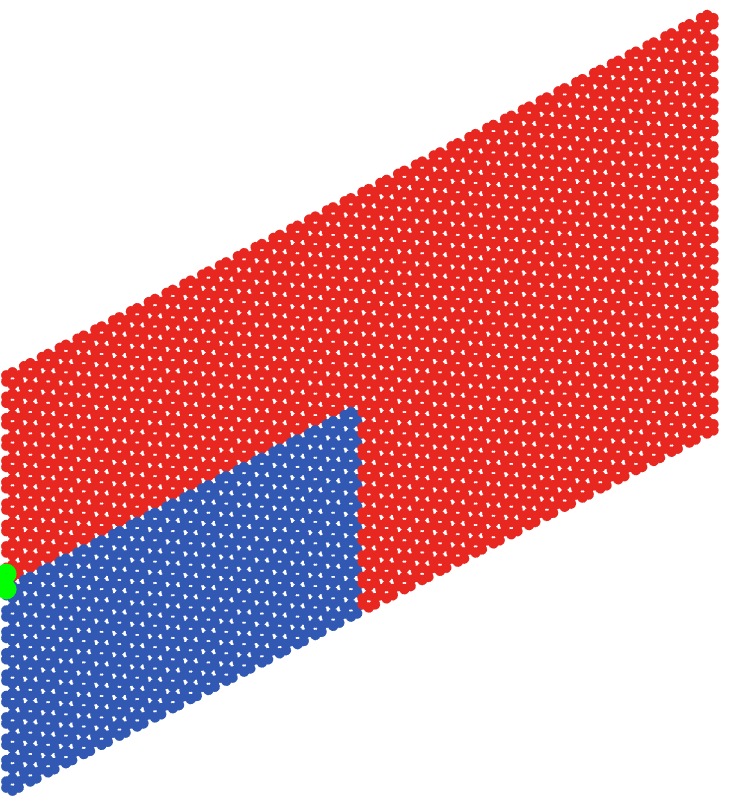
\includegraphics[width=0.8\linewidth]{imgs/sharpbendarr.png}
  \caption{Arrangement of cells to form a sharp bend.}
  \label{fig:sub1}
\end{subfigure}%
\begin{subfigure}[b]{.5\textwidth}
  \centering
  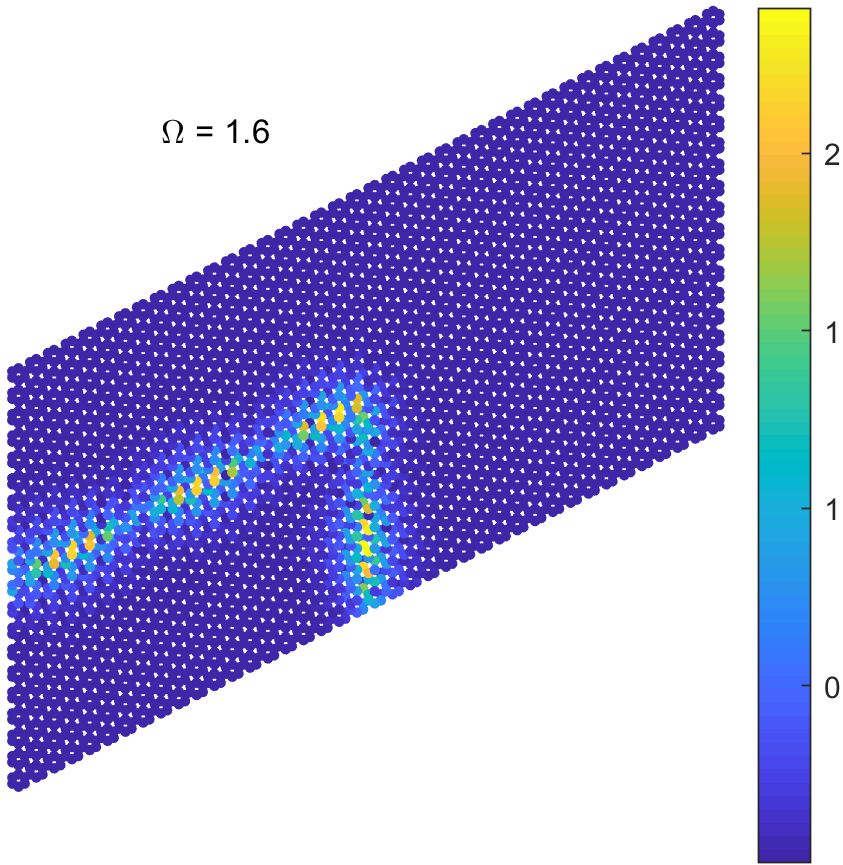
\includegraphics[width=1\linewidth]{imgs/sharpbendscat.png}
  \caption{The plot of $|y_i|$ for each mass in each cell.}
  \label{fig:sub2}
\end{subfigure}
\caption{Simulation of scattering on the hexagonal finite lattice with sharp
  bend.}
\label{fig:sharpbend}
\end{figure}

Amazingly, our system is able to stand up to both of these bends as we can see
in Figure~\ref{fig:gentlebend} and Figure~\ref{fig:sharpbend}.

%TODO: Continue with combination of straight bends; cross/interlace etc

\subsection{Curved bends}
So it can travel around gentle and sharp straight bends; it is only natural to
then wonder if it can propagate as well along a curved bend.

\begin{figure}
\centering
\begin{subfigure}[b]{.5\textwidth}
  \centering
  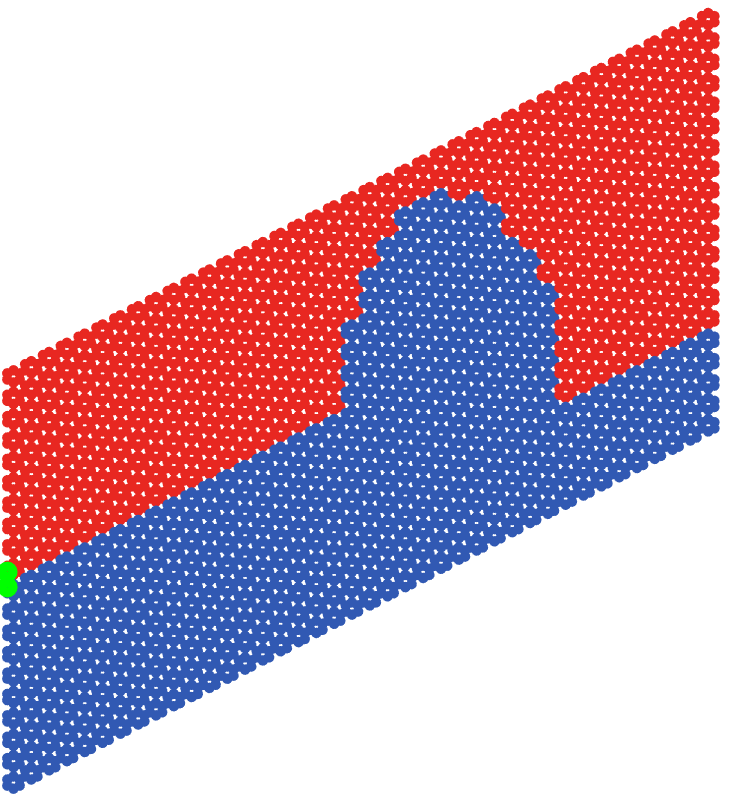
\includegraphics[width=0.8\linewidth]{imgs/curvedbendarr.png}
  \caption{Arrangement of cells to form a curved bend.}
  \label{fig:sub1}
\end{subfigure}%
\begin{subfigure}[b]{.5\textwidth}
  \centering
  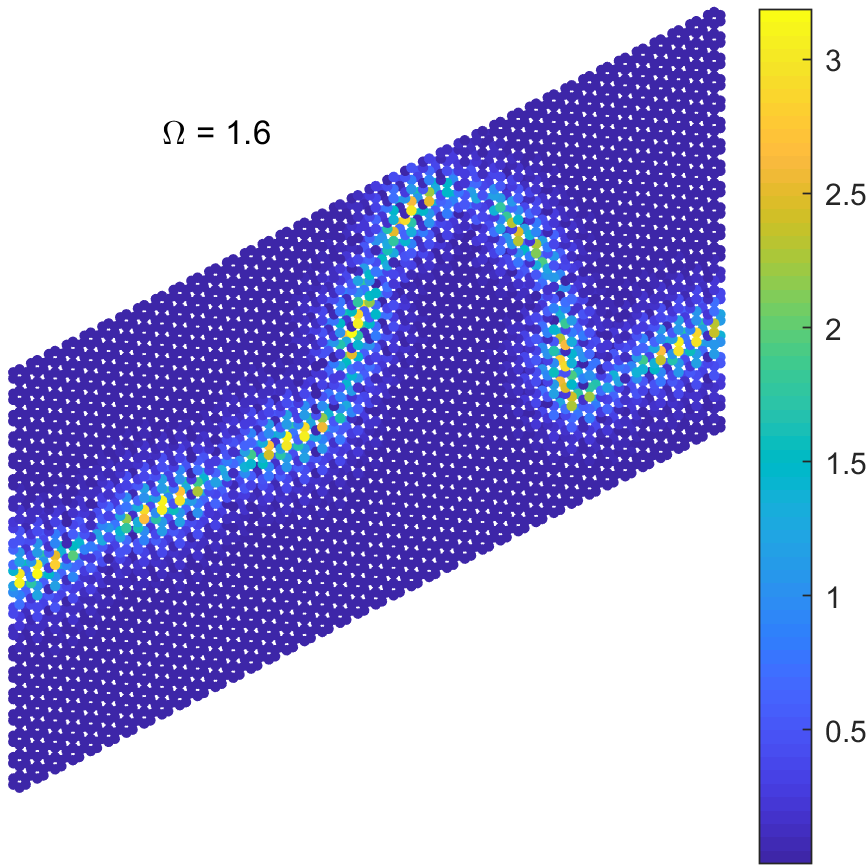
\includegraphics[width=1\linewidth]{imgs/curvedbendscat.png}
  \caption{The plot of $|y_i|$ for each mass in each cell.}
  \label{fig:sub2}
\end{subfigure}
\caption{Simulation of scattering on the hexagonal finite lattice with curved
  bend.}
\label{fig:curvedbend}
\end{figure}

\subsection{Grading}
